\documentclass{article}
\usepackage{amsmath,amsfonts}
\usepackage{tikz}
\usepackage{graphicx}
\usepackage{float}
\usepackage{booktabs}

\begin{document}

\title{Finite Difference Solution of the 1D Advection Equation}
\author{}
\date{}
\maketitle

\section*{1. Governing Equation}

The one-dimensional advection equation describes the transport of a scalar quantity $u(x,t)$ with a constant velocity $c$:
\begin{equation}
\frac{\partial u}{\partial t} + c \frac{\partial u}{\partial x} = 0.
\tag{A}
\end{equation}

This equation states that the rate of change of $u$ at a point is balanced by its spatial transport due to the velocity $c$.

\vspace{0.5em}
\noindent\textbf{Definition.}  
**Advection** is the process by which a physical quantity is transported by the bulk motion of a fluid or wave.

---

\section*{2. Discretization of the Equation}

We discretize both time and space using finite differences:

\begin{itemize}
  \item Let $x_i = i \Delta x$ for $i = 0, 1, ..., N$ be the spatial grid points.
  \item Let $t^j = j \Delta t$ for $j = 0, 1, 2, ...$ be the time levels.
  \item Denote $U_i^j \approx u(x_i, t^j)$.
\end{itemize}

\begin{figure}[H]
\centering
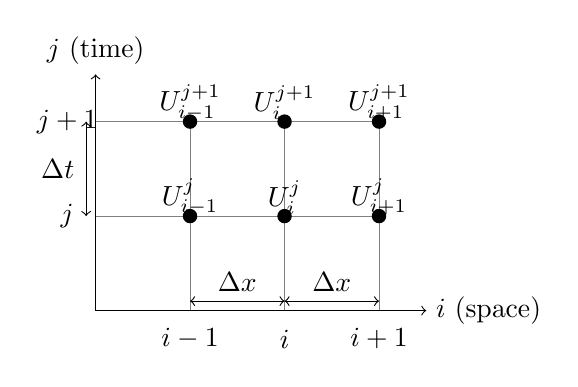
\begin{tikzpicture}[scale=1.2]
  % Grid lines
  \draw[step=1cm,gray,very thin] (0,0) grid (3,2);

  % Axes
  \draw[->] (0,0) -- (3.5,0) node[right] {$i$ (space)};
  \draw[->] (0,0) -- (0,2.5) node[above] {$j$ (time)};

  % Labels
  \node at (1, -0.3) {$i-1$};
  \node at (2, -0.3) {$i$};
  \node at (3, -0.3) {$i+1$};

  \node at (-0.3, 1) {$j$};
  \node at (-0.3, 2) {$j+1$};

  % Points
  \foreach \x in {1,2,3} {
    \foreach \y in {1,2} {
      \filldraw[black] (\x,\y) circle (2pt);
    }
  }

  % Labels
  \node at (1, 1.2) {$U_{i-1}^{j}$};
  \node at (2, 1.2) {$U_{i}^{j}$};
  \node at (3, 1.2) {$U_{i+1}^{j}$};

  \node at (1, 2.2) {$U_{i-1}^{j+1}$};
  \node at (2, 2.2) {$U_{i}^{j+1}$};
  \node at (3, 2.2) {$U_{i+1}^{j+1}$};

  % Δx
  \draw[<->] (1, 0.1) -- (2, 0.1);
  \node at (1.5, 0.3) {$\Delta x$};
  \draw[<->] (2, 0.1) -- (3, 0.1);
  \node at (2.5, 0.3) {$\Delta x$};

  % Δt
  \draw[<->] (-0.1, 1) -- (-0.1, 2);
  \node at (-0.4, 1.5) {$\Delta t$};
\end{tikzpicture}
\caption{Finite difference formulation showing the implicit time and central space discretization for the advection equation.}
\end{figure}


We approximate the partial derivatives as follows.

---

\subsection*{2.1. Time Derivative (Implicit Scheme)}

Using the backward difference in time:
\begin{equation}
\left. \frac{\partial u}{\partial t} \right|_i^{j+1} \approx \frac{U_i^{j+1} - U_i^j}{\Delta t}.
\tag{B}
\end{equation}

This is known as the **implicit (backward Euler) time discretization**, which is unconditionally stable for linear problems.

---

\subsection*{2.2. Spatial Derivative (Central Difference)}

We approximate the spatial derivative at the new time level $j+1$ using a centered difference:
\begin{equation}
\left. \frac{\partial u}{\partial x} \right|_i^{j+1} \approx \frac{U_{i+1}^{j+1} - U_{i-1}^{j+1}}{2 \Delta x}.
\tag{C}
\end{equation}

---

\section*{3. Substitution into the Governing Equation}

Substituting Equations (B) and (C) into Equation (A) gives:
\[
\frac{U_i^{j+1} - U_i^j}{\Delta t} + c \cdot \frac{U_{i+1}^{j+1} - U_{i-1}^{j+1}}{2 \Delta x} = 0.
\tag{D}
\]

---

\section*{4. Rearrangement}

Rearrange Equation (D) to solve for $U_i^{j+1}$:

\[
U_i^{j+1} - U_i^j + \frac{c \Delta t}{2 \Delta x} (U_{i+1}^{j+1} - U_{i-1}^{j+1}) = 0.
\]

Define the Courant-like parameter:
\[
\lambda = \frac{c \Delta t}{2 \Delta x}.
\tag{E}
\]

Then Equation (D) becomes:
\[
U_i^{j+1} + \lambda U_{i+1}^{j+1} - \lambda U_{i-1}^{j+1} = U_i^j.
\tag{F}
\]

---

\section*{5. Final Discrete Update Equation}

Thus, at each interior grid point $i$, we solve:
\[
-\lambda U_{i-1}^{j+1} + U_i^{j+1} + \lambda U_{i+1}^{j+1} = U_i^j.
\tag{G}
\]

This forms a tridiagonal linear system for all $U^{j+1}$.

\vspace{0.5em}
\noindent\textbf{Definition.}  
A **tridiagonal system** is a linear system in which each equation only involves a variable and its two immediate neighbors.

---

\section*{6. Matrix Representation}

The system for all grid points can be written in matrix form:

\[
A \mathbf{U}^{j+1} = \mathbf{U}^j,
\quad
A \in \mathbb{R}^{N \times N}.
\tag{H}
\]

Where $A$ is a tridiagonal matrix:
\[
A =
\begin{pmatrix}
1 & \lambda/2 & 0 & \cdots & 0 \\
-\lambda/2 & 1 & \lambda/2& \cdots & 0 \\
0 & -\lambda/2 & 1 & \lambda/2 & 0 \\
\vdots & \ddots & \ddots & \ddots & \vdots \\
0 & \cdots & 0 & -\lambda/2 & 1
\end{pmatrix}.
\]


\end{document}
